\chapter{Compositionality for Safe-by-construction ML-based Cyber-Physical Systems} \label{chapter:av}
\glsresetall




\section{Overview}

In light of the problems with the verification of ML-based CPS, as highlighted in Chapters \ref{chapter:background} and \ref{chapter:lit_review}, in this chapter, we present a framework that extends the compositional framework discussed in Chapter \ref{chapter:compositional} to design an ML-based CPS that is safe by construction. We propose learning formally defined policies from realistic data and using them to guide training and deployment. While some recent works have explored policy mining in the context of ML \cite{10.5555/1625015.1625078, panda_explainable_2024}, to the best of our knowledge, no existing methodology leverages these mined policies to train compositional ML models to ensure policy compliance and system-level safety. With this work, we make the following contributions.
\begin{itemize}
    \item We present a novel policy mining framework that derives safety rules or policies from real-world data using defined policy templates. 
    \item We introduce a policy-guided compositional model development and training methodology for ML-based CPS for the first time. We extend the work in the previous chapter by exploring a more complex model architecture and different types of ML models.
    \item We develop runtime enforcers to detect and mitigate policy violations in real-time, providing an additional safety net for unmodeled conditions.
    \item We validate our approach on a comprehensive AV case study, demonstrating improved safety guarantees and competitive performance.
\end{itemize}

 
The remainder of this chapter is organised as follows. Section~\ref{sec:motivating_example} motivates our approach with a driving scenario that challenges monolithic models. Section~\ref{sec:compositional_training} details our compositional training method. Section~\ref{sec:runtime_enforcement} presents our runtime enforcement strategies. In Section~\ref{sec:case_study}, we report on our AV experiments. Section~\ref{sec:results} presents training and simulation outcomes and includes a discussion of their implications. Finally, Section~\ref{sec:av_summary} summarises the chapter.



\section{Motivating example}
\label{sec:motivating_example}
Consider the safety-critical example of an AV. We can design a simple AV comprised of different modules that work on different tasks (as shown in Figure \ref{fig:av}). This compositional architecture comprises multiple modules implemented using different mathematical models, such as ANN models or others. %Compositionality allows for the separation of concerns and easier maintenance of modules, which is difficult in a single-module (monolithic) architecture. 
The following is a brief description of the modules in the AV design.

\begin{itemize}
 \item \gls{lcd} module, which is responsible for deciding when it is safe to change lanes,
 \item \gls{cf} module that controls the car following behaviour; it is responsible for maintaining a safe distance from the car in front;
 \item \gls{lce} module, which is responsible for executing the lane change;
 \item Controller module, which assists in changing between the three aforementioned modes;
\item Runtime enforcers \cite{pearce_smart_2020,10.1145/3126500} after each module to guarantee its behaviour. The enforcer checks the output of the module and ensures that it satisfies the required policies. Their addition ensures that only correct outputs are sent to the controller module.
\item The AV is also equipped with a perception module that uses sensors to detect the environment and other vehicles and provide these inputs to the modules. 
\end{itemize}

%In this case study, we consider the \gls{lcd} module implemented as a compositional ANN model.
\begin{figure}[htbp]
 \centering
 
\includegraphics[width=\linewidth]{av_case_study/fig/AV_full.pdf}
 \caption{AV case study}
 \label{fig:av}
\end{figure}

\noindent \textit{Intuition on Compositionality of modules}:
If we take the example of the \gls{lcd} module, all three lanes are typically considered during a lane change: the lane the vehicle is currently in and the lanes to its left and right, if available. A human driver would first observe the car ahead to decide if a lane change is necessary, then check the left and right lanes to ensure that there is a safe space to perform the manoeuvre. Thus, the monolithic \gls{lcd} module can be further decomposed into submodules: one for the "\textit{Opportunity model}" to assess whether a lane change is advisable or necessary, one for the "\textit{Left \gls{lc}}" model to evaluate the safety of a left lane change, and one for the "\textit{Right \gls{lc}}" model to evaluate the safety of a right lane change. This decomposition demonstrates the significance of modularisation for better functionality and analysis.\vspace{0.5em}


\noindent \textit{Intuition on Compositionality of policies}: We need to guarantee certain system-level behaviours/policies for the AV, and designing these policies compositionally can be beneficial as well. System-level policies can be defined and decomposed across modules to simplify verification. For example, an AV with three modules can have a system-level "\textit{No collision}" policy decomposed into sub-policies such as "\textit{No collision due to \gls{lcd}} ", "\textit{No collision due to CF}", and "\textit{No collision due to \gls{lce}} ". The policy for the \gls{lcd} module can be further decomposed and divided across the submodules as discussed previously. This way, the overarching policy, expressed as maintaining sufficient gaps between the AV and adjacent vehicles, can be distributed across various modules for more manageable analysis and enforcement. 

In the following sections, we discuss how we can design compositional modules and policies and train such modules with their policies for the AV case study.


\begin{figure*}[htbp]
   \centering
   
\includegraphics[width=\linewidth]{/Users/sobhanchatterjee/Desktop/PAPERS/Papers/UoA Thesis/sections/av_case_study/fig/Methodology_training.pdf}
   \caption{The whole compositional policy-driven training methodology.}
        \label{fig:pol_driven_training}
  \end{figure*}
    
  


\section{Policy-driven Model Development}
\label{sec:compositional_training}

\subsection{Overview}
\label{sec:comp_overview}
Our methodology begins by defining a compositional policy template that specifies the desired structure of policies to be mined  (see Figure \ref{fig:pol_driven_training}). The policies are expressed as predicate-logic formulas. A compositional policy mining process extracts modular policy components from the data using this template. Real-world data is used to guide this process, ensuring that the mined policies reflect actual conditions. A corresponding compositional model is then designed from the mined compositional policy. The model undergoes compositional training using a filtered dataset that conforms to the policy template and is suitable for deployment or further refinement.

To motivate our approach, consider an autonomous driving scenario where an ego/subject vehicle must decide whether to change lanes when it is surrounded by six surrounding vehicles (two in front and back, and two each on either lane). This decision depends on the dynamic configuration of surrounding vehicles, such as nearby cars' relative distances, velocities, and accelerations.

As an example, a safety policy might state:
\begin{quote}
\emph{The ego vehicle may initiate a left lane change only if the gap to the left-front vehicle is sufficiently large, given their relative speed and acceleration.}
\end{quote}

This policy can be formalised using predicate logic, with parameters to be learned from data. Let $y$ denote the configuration of the environment, and let $\varphi_{LF}(y)$ encode the safety condition for the left-front vehicle. Then:
\begin{equation}
 \varphi_{LF}(y)
 \;\equiv\;
 lfX \;>\; (b_0 lfV + b_1 lfA + b_2),
\label{eq:lf_policy}
\end{equation}
where:
\begin{itemize}
  \item $y = \{\,lfX, lfV, lfA,\dots, rpX, rpV, rpA, \dots, bX, bV, bA\}$ encodes the real-time relative distances, velocities, and accelerations between the ego vehicle and each of the six surrounding vehicles.  
  \item $lfX$, $lfV$, $lfA$ are extracted from $y$
  \item $b_0, b_1, b_2$ are parameters to be learned from data.
\end{itemize}

This policy expresses that the left-front gap $lfX$ must exceed a learned threshold computed as a linear function of the velocity and acceleration. The values of AV configurations ($y$) are obtained from the highD dataset \cite{krajewski_highd_2018}, which contains trajectory data of multiple vehicles recorded on German highways, providing examples of real driving interactions from which we can learn safety and gap-keeping rules. We now describe the formal structure used to define such policies.


 

% (Removed the paragraph that was flagged as unnecessary by Partha.)

%% ------------------------------------------------------------------------

\subsection{Compositional Policies}
\label{sec:compositional_policies}
We recall standard predicate-logic definitions in this section, derived from \cite{10.5555/2974990}. We need to define terms and atoms, which are the basic building blocks of predicate logic. \vspace{0.5em}

\noindent \textit{Term}: A term is defined inductively as follows:
\begin{enumerate}
    \item A variable is a term.
    \item A constant is a term.
    \item If \( f \) is a function symbol and \( t_1, \ldots, t_n \) are terms, then \( f(t_1, \ldots, t_n) \) is a term.
    \item Nothing else is a term.
\end{enumerate}

\noindent \textit{Atom}: An atom (or atomic formula) is defined as follows: If \( P \) is an \( n \)-place predicate symbol and \( t_1, \ldots, t_n \) are terms, then \( P(t_1, \ldots, t_n) \) is an atomic formula (or atom).\vspace{0.5em}

\noindent \textit{Well-formed formula (wff)}: A wff (or just a formula) is defined inductively as follows:
\begin{enumerate}
    \item An atom is a wff.
    \item If \( \varphi_1\) and \( \varphi_2\) are wffs, then the following are also wffs:
    \[
 \lnot \varphi_1,\quad 
 \varphi_1 \land \varphi_2,\quad 
 \varphi_1 \lor \varphi_2,\quad 
 \varphi_1 \rightarrow \varphi_2
    \]
    \item If \( \varphi \) is a wff and \( x \) is a variable, then the following are wffs:
    \[
 (\forall x)\, \varphi,\quad (\exists x)\, \varphi
    \]
    \item Nothing else is a wff.
\end{enumerate}

The above can also be seen in the Backus-Naur Form (BNF) for predicate logic:
\[
 \varphi ::= P(t_1, t_2, \ldots, t_n) 
 \mid \lnot \varphi 
 \mid (\varphi \land \varphi) 
 \mid (\varphi \lor \varphi) 
 \mid (\varphi \rightarrow \varphi) 
 \mid (\forall x\, \varphi) 
 \mid (\exists x\, \varphi)
\]

\vspace{0.5em}
\noindent \textit{Semantics}: Interpretation of a formula in a non-empty domain $D$ is achieved by assigning values to constant symbols (to each constant assign an element of $D$), function symbols (to each $n$-place function symbol assign a mapping $D^n \!\to\! D$) and predicate symbols (to each $n$-place predicate symbol assign a mapping $D^n \!\to\! \{\mathsf{T},\mathsf{F}\}$).

\vspace{0.5em}
\noindent \textit{Satisfiability}: A formula $\varphi$ is satisfiable if and only if there exists an interpretation $I$ such that $\varphi$ evaluates to true under $I$:
\[
 \varphi \text{ is satisfiable}
 \quad\Longleftrightarrow\quad
 \exists I \;\text{such that}\; I \models \varphi.
\]


\begin{example}[Interpreting an AV policy as a logical formula]
\label{example:lf_policy_logic}

Reusing the policy stated in Equation \ref{eq:lf_policy}, we can explain it in light of the current formalism as follows.
\begin{equation}
 \underbrace{\varphi_{LF}(y)}_{\substack{\text{Predicate over}\\\text{configuration }y}}
 \;\equiv\;
 \underbrace{lfX}_{\text{Term: gap to left-front}}
 \;>\;
 \underbrace{b_0\vphantom{lfX}\,lfV 
 \;+\;b_1\,lfA 
 \;+\;b_2}_{\text{Term: learned linear function}},
  \label{eq:lf_policy_2}
\end{equation}
where:
\begin{itemize}
  \item $y$ is the state vector including $\{lfX,lfV,lfA,\dots\}$,
  \item $lfX,lfV,lfA$ are \emph{terms} extracted from $y$ (gap, relative velocity, relative acceleration),
  \item $b_0,b_1,b_2$ are constant coefficients \emph{learned} from the highD dataset,
  \item $>$ is a binary predicate symbol forming an \emph{atomic formula}.
\end{itemize}

According to the syntax of predicate logic:
\begin{itemize}
  \item Each of $lfX,lfV,lfA$ is a \emph{term},
  \item The expression $b_0\,lfV + b_1\,lfA + b_2$ is a \emph{term},
  \item The full formula $lfX > (b_0 lfV + b_1 lfA + b_2)$ is an \emph{atomic formula} $P(t_1,t_2)$.
\end{itemize}

Thus, $\varphi_{LF}(y)$ is a \emph{well-formed formula (wff)}.

$\varphi_{LF}(y)$ holds under an interpretation $I$ if and only if
\[
 I \models \varphi_{LF}(y)
 \quad\Longleftrightarrow\quad
 I(lfX) > I(b_0\,lfV + b_1\,lfA + b_2).
\]
That is, the actual left-front gap exceeds the learned threshold. $\square$
\end{example}

%% ------------------------------------------------------------------------

\begin{definition}[Compositional Policy]
\label{def:compositional_policy}
A compositional policy $\varphi$ is a wff that combines simpler policies (or rules) $\varphi_1,\dots,\varphi_n$ using logical operators and/or quantifiers. Each constituent must itself be a wff.

Formally, let $\varphi_1,\dots,\varphi_n$ be wffs.  Then:
\[
 \varphi ::= \varphi_i
 \mid \lnot \varphi
 \mid (\varphi_1 \land \varphi_2)
 \mid (\varphi_1 \lor \varphi_2)
 \mid (\varphi_1 \rightarrow \varphi_2).
\]
\end{definition}


\begin{example}[Lane-change decision policy: a compositional policy]
\label{example:compositional_policy_av}

%--- Scenario description
Continuing the autonomous driving scenario from Section \ref{sec:comp_overview}, we define the compositional policy for a lane change. At each decision step, the ego vehicle observes its dynamic \emph{configuration} $y$, which includes the relative distances, velocities, and accelerations of these six neighbours.


We begin by defining six \emph{atomic} policies, each of which checks a "safe-gap" condition against one of the six neighbours:
\[
 \varphi_{LF}(y),\;
 \varphi_{LP}(y),\;
 \varphi_{RF}(y),\;
 \varphi_{RP}(y),\;
 \varphi_{F}(y),\;
 \varphi_{B}(y)
\]
Here, for example, $\varphi_{LF}(y)$ ($y=\{lfX, lfV, lfA\}$) asserts that the gap to the left-front vehicle exceeds a learned threshold, while $\varphi_{RP}(y)$ ($y=\{rfX, rfV, rfA\}$) asserts that the gap to the right-rear vehicle is safe, and so on.

%--- Composite policy formula
Intuitively, the ego may change lanes to the left if both left-front and left-rear gaps are safe (safe left lane change) or to the right if both right-front and right-rear gaps are safe (safe right lane change)—and in either case, there must also be a sufficient gap in the current front and rear directions (opportunity) to ensure safe manoeuvre:
\begin{equation}
 \varphi_{\gls{lcd}}(y)
 \;=\;
 [\bigl(\varphi_{LF}(y)\land\varphi_{LP}(y)\bigr)
 \;\lor\;
 \bigl(\varphi_{RF}(y)\land\varphi_{RP}(y)\bigr)]
 \;\land\;
 \bigl(\varphi_{F}(y)\land\varphi_{B}(y)\bigr)
  \label{eq:phi_LCD}
\end{equation}

By Definition~\ref{def:compositional_policy}, this composite policy $\varphi_{\gls{lcd}}(y)$ is a well-formed formula and is \emph{satisfiable} precisely when there exists some configuration $y$ (and an interpretation of any learned parameters) such that
\[
 I \models \varphi_{\gls{lcd}}(y),
\]
i.e.\ all of the required safe-gap conditions hold simultaneously for that state. The next section explains how the parameters for the linear functions used in the policy predicates can be mined from data. $\square$
\end{example}






\subsection{Policy Mining from Data}
\label{sec:policy_mining}



\begin{algorithm}[htbp]
   \caption{Policy-mining approach}
   
   \begin{algorithmic}[1]
    \State \textbf{Input:} Dataset $\mathcal{\mathbf{D}} = \{(\mathbf{X}_i, \mathcal{A}_i)\}_{i=1}^N$ based on the policy template $\varphi_l$, where $\mathbf{X}_i$ are features and $\mathcal{A}_i$ are label values. Target satisfaction percentage $\mathcal{T}$, maximum iterations $\mathcal{I}$.
    \State \textbf{Output:} Optimized parameters $\tilde{\mathbf{B}}$, satisfaction percentage $\mathcal{S}$, and indices $\mathcal{I}_{\text{sat}}$ of satisfying datapoints.
       
    % \State \textbf{Step 1: Property Definition}
    % \State Define the policy template as an inequality:
    %    \[
    % \varphi_i : \mathcal{A} - (\mathbf{X}_i \mathbf{B}) \geq 0
    %    \]
    % where $\mathcal{A}$ is a threshold and $\mathbf{B}$ are parameters to optimize.
    \Statex 
    \State \textbf{Step 1: Initial parameter Estimation via \gls{ols}}
    \State Fit an gls{ols} model using $\mathcal{\mathbf{D}}$ to obtain initial parameters $\hat{\mathbf{B}}$:
       \[
    \hat{\mathbf{B}} = \underset{\mathbf{B}}{\arg\min} \sum_{i=1}^N \left( \mathcal{A}_i - \mathbf{X}_i \mathbf{B} \right)^2
       \]
     \Statex  
    \State \textbf{Step 2: Optimization}
    \State Set the initial threshold $\mathcal{A}_{\text{fixed}}$ as:
       \[
    \mathcal{A}_{\text{fixed}} = \sum_{j=1}^k \hat{B}_j \cdot \text{mean}(\mathbf{X}_j) - \min(\mathcal{A})
       \]
    \State Define the objective function $\mathcal{F}(\mathbf{B})$:
       \[
    \mathcal{F}(\mathbf{B}) = \frac{1}{N} \sum_{i=1}^N \mathbf{1}\left(P \text{ is satisfied for } (\mathbf{X}_i, \mathcal{A}_i)\right)
       \]
    \State Perform optimisation using  \gls{bfgs}:
       \[
    \tilde{\mathbf{B}} = \underset{\mathbf{B}}{\arg\min} \left(\sum_{i=1}^N \left(\mathcal{A}_i - (\mathbf{X}_i \mathbf{B} \pm \mathcal{A}_{\text{fixed}})\right)^2 \right)
       \]
    Stop early if $\mathcal{F}(\tilde{\mathbf{B}}) \geq \mathcal{T}$.
    \State Return $\tilde{\mathbf{B}}$, $\mathcal{F}(\tilde{\mathbf{B}})$, and satisfying indices $\mathcal{I}_{\text{sat}}$.
    \end{algorithmic}
       \label{alg:compositional_training}
   \end{algorithm}
   
   
   
The policy mining methodology is shown in Algorithm \ref{alg:compositional_training}. Here, the algorithm assumes as input the following:
\begin{itemize}
    \item a wff compositional policy ($\varphi$) with constituent policies $\varphi_l$, which are wff. We assume that all wff policies have a fixed template of a linear inequality (with some parameters to be estimated). It is an inequality of the form:
 \begin{equation}
 \varphi_l : \mathcal{A}_i - (\mathbf{X}_i \mathbf{B}) \geq 0,
 \end{equation}
 where $\mathcal{A}_i \in \mathbb{R}$ and $\mathbf{X}_i \in \mathbb{R}^k$ are both obtained from a dataset, $\mathbf{B} \in \mathbb{R}^{(k+1) \times 1}$ (where $k$ is the number of features or predictors) is the set of parameters to be optimised, and $i$ refers to the $i^{th}$ datapoint;

    \item a dataset $\mathcal{\mathbf{D}}$ consisting of features ($\mathbf{X} \in \mathbb{R}^{N \times (k+1)}$, where $k+1$ is the number of features and intercept, and N is the number of datapoints) and the corresponding label values ($\mathcal{A}$), extracted based on the policy template;
   
   \item a target satisfaction percentage $\mathcal{T}$, e.g.\ 98\%, used both to measure how often the policy holds on the training set and to trigger early stopping once reached.

 \smallskip
 \noindent\emph{Note:}  Choose $\mathcal{T}<100\%$ to allow for modelling noise and ensure enough positive and negative examples, balancing high satisfaction with generalisation;


    \item a maximum number of iterations $\mathcal{I}$ (we need a maximum number of iterations even with a target satisfaction percentage because the target might never be reached). 
\end{itemize}

The algorithm outputs the learned template parameters $\tilde{\mathbf{B}} = \{\tilde{b}_1,\dots,\tilde{b}_k\}$, the empirical satisfaction rate $\mathcal{S}$—which may fall below or exceed the target $\mathcal{T}$ depending on data granularity—and the index set $\mathcal{I}_{\mathrm{sat}}$ of all datapoints that satisfy the mined policy.


Now, once we get the initial estimation, the algorithm sets a fixed threshold $\mathcal{A}_{\text{fixed}}$. Essentially, \( \mathcal{A}_{\text{fixed}} \) sets a baseline value that adjusts the inequality  $\mathcal{A}_i - (\mathbf{X}_i \mathbf{B}) \geq 0$ so that the decision boundary reflects both the central tendency of the feature data and the lower bound of the labels. This calibration ensures that the subsequent optimisation is feasible and that the model is not overly restrictive. 

Also, to guide the optimisation process, the objective function $\mathcal{F}(\mathbf{B})$ is defined as in line 7 of the algorithm, where the indicator function $\mathbf{1}$ determines whether the policy condition holds for a given data point. The goal is to maximise this function while refining the parameters. The algorithm employs the  \gls{bfgs} optimisation algorithm \cite{doi:https://doi.org/10.1002/9781118723203.ch3} to minimise the Mean Squared Error (MSE) between the predicted and actual value of $\mathcal{A}$. The optimisation continues until the satisfaction function $\mathcal{F}(\tilde{\mathbf{B}})$ reaches or exceeds the target percentage $\mathcal{T}$, at which point the process terminates early. This step is repeated for each wff in the overall policy ($\varphi$).


\vspace{0.5em}
\noindent \textit{Note} (Repeated Optimisation for Each wff):
Algorithm \ref{alg:compositional_training} is repeated for each $\varphi_l$ in the compositional policy $\varphi$, ensuring that each policy component is optimised to maximise satisfaction.


\begin{example}[Policy Mining for the AV example]
\label{example:compositional_policy_template}
Continuing Example~\ref{example:compositional_policy_av}, we assume that Equation \ref{eq:phi_LCD} defines the compositional policy. The constituent policy formulae (as shown in Equation \ref{eq:lf_policy_2}) can be seen as a learned instantiation of the classical kinematic inequality:

The classical kinematic gap condition can be written as: 
\begin{equation}
 \text{gap} \;>\; v\,t \;+\; \tfrac{1}{2} a\,t^2,
  \label{eq:uniform_motion_ref}
\end{equation}
where \textit{gap} is the required safe distance between vehicles, $v$ is the relative velocity, $a$ is the relative acceleration, and $t$ is the reaction time. This formula ensures that the following vehicle has enough space to react safely to changes in traffic.

In this interpretation, we identify $\text{gap}=lcfX$, $v = lfV$ and $a = lfA$. All other gap conditions, such as $\varphi_{LP}(y)$, $\varphi_{RF}(y)$, etc., are defined using analogous templates with corresponding feature subsets from $y$. 

Thus, for the AV example, the algorithm \ref{alg:compositional_training} uses the dataset $\mathbf{D}$ obtained by extracting features $X_i = \{lcfV,  lcfA,...,bV,bA\}$, which contain the velocities and accelerations of cars, and labels $\mathcal{A}_i = \{lcfX,rcfX,...,fX,bX\}$, which contains the relative gaps of cars, from the highD dataset from cars that lane change. The algorithm is then run with a certain target satisfaction percentage $\mathcal{T}$ and satisfaction percentage $\mathcal{S}$ for each $\varphi_i \equiv \varphi_{LF},...,\varphi_{B}$ to obtain the optimised values of the unknown coefficients ($b_0, b_1, b_2$).

$\square$
\end{example}

The policy predicates in Equation \ref{eq:lf_policy_2} are not just learned from data. The \emph{structure} of each constituent policy---which variables appear, the linear inequality template, and its connection to domain knowledge such as the kinematic gap condition in Equation \ref{eq:uniform_motion_ref}---is fixed by the system designer before mining. Data is used to estimate the unknown coefficients ($b_0, b_1, b_2$, etc.) and to calibrate how often the predicate holds on real trajectories. We set the target satisfaction percentage $\mathcal{T}$ below 100\% because highway recordings contain sensor noise, labelling uncertainty, and borderline manoeuvres; a strict 100\% target would overfit rare outliers and leave too few counterexamples for training. The mined parameters therefore \emph{augment} domain knowledge by fitting the template to empirical conditions (e.g.\ highD), rather than replacing first-principles constraints. In our AV case study, the template is grounded in gap--velocity--acceleration relationships. Coefficients that produce systematically unsafe gaps can be rejected by inspection, by holding out validation data. Ultimately, the runtime enforcer, as we discuss in Section \ref{sec:runtime_enforcement}, guarantees adherence to the mined policy at deployment regardless of ML prediction errors.


\subsection{Compositional Model Design}
\label{sec:model_decomposition}

Often, compositional policies are defined using a monolithic (a single large) ML model. In such instances, it is prudent to decompose the monolithic model into a compositional model. We propose a novel approach that allows decomposing a monolithic model based on the compositional policy that the monolithic model must satisfy. This approach is model-agnostic and can be used with any ML model. 

\begin{definition}[Compositional Multilevel Decomposition]
 Let $\mathcal{X}$ and $\mathcal{Y}$ denote the input and output spaces, respectively. A monolithic ML model is a function 
    \[
 M \colon \mathcal{X} \to \mathcal{Y}.
    \]
\sloppy Given a compositional policy $\varphi$ as defined earlier in Definition \ref{def:compositional_policy}, expressed as a wff over a set of simpler policies $\{\varphi_1, \varphi_2, \dots, \varphi_n\}$, the decomposition of $M$ into $\{M_1, M_2, \dots, M_k\}$ is structured as a tree with leaf nodes and internal nodes. It is defined as follows.\vspace{0.5em} 
   
\noindent \textbf{Leaf Nodes of the Compositional Architecture:} 
Each leaf node $l$ corresponds to a well-formed formula (wff) $\varphi_l$. This wff may be atomic or itself a composite formula constructed using logical connectives (e.g., $\land$, $\lor$) over a finite set of sub-formulae $\{\varphi_i, \ldots, \varphi_j\}$. The node is associated with a sub-model
\[
M_l \colon \mathcal{X} \to \mathcal{Y}_l,
\]
which maps input configurations to a semantic domain $\mathcal{Y}_l$ over which the formula $\varphi_l$ is interpreted.

We say that the sub-model $M_l$ satisfies $\varphi_l$ under interpretation $I$ with respect to a set of inputs $\mathcal{X}_{\text{val}} \subset \mathcal{X}$ if
\[
\forall x \in \mathcal{X}_{\text{val}}, \quad I \models \varphi_l\big(M_l(x)\big).
\]
In practice, this is relaxed to approximate satisfaction, where we compute the empirical proportion of inputs for which the interpretation satisfies the formula:
\[
\frac{|\{x \in \mathcal{X}_{\text{val}} \mid I \models \varphi_l(M_l(x)) \}|}{|\mathcal{X}_{\text{val}}|} \geq P_l,
\]
for some target percentage $P_l \in [0, 1]$.

The leaf nodes are the sub-models that will be trained to satisfy their respective formulae $\varphi_l$ under this semantic framework.



\vspace{0.5em}
 \noindent \textbf{Internal Nodes of the Compositional  architecture:} Each internal node $v$ of the compositional  architecture represents a \textit{Merge} block. 
 The \textit{Merge} block combines two wffs using a specified connective $op \in \{\land, \lor\}$, based on the given policy.
    \[(X,Y,op)=X ~op~ Y\]
where $X,Y$ are wffs and $op \in \{\land, \lor\}$ is determined by the policy. $\square$

\end{definition}

  

The structure of the compositional policy guides the architecture of the decomposed system. Leaf nodes represent sub-models satisfying wff, while internal nodes combine the outputs of the leaf nodes or other internal nodes. 


\begin{figure}[htbp]
 \centering
 
\includegraphics[width=\linewidth]{/Users/sobhanchatterjee/Desktop/PAPERS/Papers/UoA Thesis/sections/av_case_study/fig/PropertiesComp.pdf}
 \caption{3-stage compositional architecture of the \gls{lcd} module.}
      \label{fig:3_stage_decomposition}
\end{figure}
  
\begin{example}(Compositional model: AV Case Study Example.)
 Let us decompose a single monolithic \gls{lcd} model (considered in Example \ref{example:compositional_policy_av}) into a compositional model. In the example, we had $\varphi_{\gls{lcd}}: [(\varphi_{LF} \land \varphi_{LP}) \lor (\varphi_{RF} \land \varphi_{RP})] \land (\varphi_{F} \land \varphi_{P})$ (with interpretation $y$). Thus, we can design the model with three leaf nodes, each with a separate model, as shown in Figure \ref{fig:3_stage_decomposition}. Each leaf node is a wff. The models we obtain are 1) the Left LC model to determine whether it is safe to execute a left lane change, 2) the Right LC model to determine whether it is safe to execute a right lane change, and 3) the Opportunity model to determine whether it is advisable/needed to perform a lane change. The leaf nodes are shown in green in the decomposed architecture in Figure \ref{fig:3_stage_decomposition}.

 Now, there will be two \textit{Merge} blocks (shown in the colour purple in Figure \ref{fig:3_stage_decomposition}) used to combine the outputs of the models at each stage: The first \textit{Merge} block combines the outputs of the Left LC and Right LC models (using a disjunction operation; disjunction of the outputs $(\varphi_{LF} \land \varphi_{LP}) $ and $ (\varphi_{RF} \land \varphi_{RP}$), and the second \textit{Merge} block combines the output of the Opportunity model and the output of the first \textit{Merge} block (using a conjunction operation; conjunction of the outputs $(\varphi_{LF} \land \varphi_{LP}) \lor (\varphi_{RF} \land \varphi_{RP}) $ and $ (\varphi_{F} \land \varphi_{P})$). The final output of the compositional architecture is the output of the second \textit{Merge} block.

 We could have also gone for a six-leaf node model, where each leaf node corresponds to wffs. However, we chose to keep it simple with three leaf nodes. %The leaf nodes are the sub-models that will be trained to satisfy their respective policies.
    $\square$
  
\end{example}

We are aware that clean decomposition is not always possible, and this is an important practical limitation. Our framework assumes that the compositional policy $\varphi$ can be written as a wff over constituent predicates, each associated with a leaf model whose outputs are checked for (approximate) satisfaction of that predicate. This applies directly when sub-policies concern distinct aspects of the same configuration $y$, as in the \gls{lcd} example, where gap conditions for individual neighbours are composed logically. 

When a policy genuinely spans several ML modules in a pipeline---for example, if a downstream module's safe operation depends on the \emph{decision} produced by an upstream module---the designer should either (i)~assign a separate compositional policy to each pipeline stage (as we do for the \gls{lcd}, lane-change execution, and car-following modules in Section \ref{sec:case_study}), with a system-level enforcer on the final control output, or (ii)~retain a monolithic policy at the pipeline level and decompose only within a stage where the wff structure is clear. Cross-module dependencies are then captured by the serial composition of modules, not by splitting a single predicate across unrelated models.


\subsection{Training of Compositional Models}
\label{sec:compositional_policy_based_training}


\begin{algorithm}[htbp]
   \caption{Compositional Policy-Based Training}
   \begin{algorithmic}[1]
   \State \textbf{Input:} Dataset $\mathcal{\mathbf{D}}$, optimized parameters $\tilde{\mathbf{B}}$, satisfying indices $\mathcal{I}_{\text{sat}}$, compositional policy $\varphi$.
   \State \textbf{Output:} Trained compositional model $M_{\text{compositional}}$ and final Accuracy $\mathcal{P}$.
      
   \State \textbf{Step 1: Data Filtering}
   \State Partition $\mathcal{\mathbf{D}}$ into subsets based on satisfaction:
      \[
   \mathcal{\mathbf{D}}_{\text{sat}} = \{(\mathbf{X}_i, y_i) \in \mathcal{\mathbf{D}} \mid \varphi \text{ is satisfied}\} 
      \]
      \[
   \mathcal{\mathbf{D}}_{\text{unsat}} = \{(\mathbf{X}_i, y_i) \in \mathcal{\mathbf{D}} \mid \neg \varphi \text{ is satisfied}\}
      \]
   \State Form the combined dataset:
      \[
   \mathcal{\mathbf{D}}_{\text{combined}} = \mathcal{\mathbf{D}}_{\text{sat}} \cup \mathcal{\mathbf{D}}_{\text{unsat}}.
      \]
      
   \State \textbf{Step 2: Leaf Model Training}
   \For {each leaf node $l$ corresponding to wff $\varphi_l$}
   \State Construct model $M_l \colon \mathcal{X} \to \mathcal{Y}_l$.
   \State Train $M_l$ on $\mathcal{\mathbf{D}}_{\text{combined}}$:
          \[
   M_l = \underset{\theta_l}{\arg\min} \sum_{(\mathbf{X}_i, y_i) \in \mathcal{\mathbf{D}}_{\text{combined}}} \mathcal{L}(M_l(\mathbf{X}_i; \theta_l), y_i),
          \]
   where $\mathcal{L}$ is the loss function.
   \EndFor
      
   \State \textbf{Step 3: Compositional Model Construction}
   \State Assemble the overall compositional model $M_{\text{compositional}}$ by connecting the trained leaf models $\{M_l\}$ using the merge connectives as defined in the compositional multilevel decomposition.
      
   \State \textbf{Step 4: Accuracy Evaluation and Update}
   \State Evaluate the accuracy $\mathcal{P}$ of $M_{\text{compositional}}$ on $\mathcal{\mathbf{D}}_{\text{combined}}$:
      \[
   \mathcal{P} = \frac{|\{(\mathbf{X}_i, y_i) \in \mathcal{\mathbf{D}}_{\text{combined}} \mid \varphi\bigl(M_{\text{compositional}}(\mathbf{X}_i)\bigr) \text{ is satisfied}\}|}{|\mathcal{\mathbf{D}}_{\text{combined}}|}
      \]
   \State Update the parameters of the leaf models and merge blocks to maximise $\mathcal{P}$ until convergence.
  \State Return $M_{\text{compositional}}$ and $\mathcal{P}$.
   \end{algorithmic}
      \label{alg:compositional_training_2}
  \end{algorithm}
  
  

Once we have the compositional model architecture and the model policies, we can train the ML models to emphasise satisfying their policies. One way to approach this problem is to check policy adherence during training and penalise the model when it does not adhere to the policy. However, this approach can be computationally expensive and may not be feasible for large datasets. Thus, we present an approach in Algorithm \ref{alg:compositional_training_2}, where we do not do policy satisfaction checks inside the training loop and instead do it at the data preprocessing stage. This approach may reduce the number of overall training data points, but it requires less time and resources to train the models.



\noindent \textit{Training algorithm}: The algorithm takes as input a training dataset $\mathcal{\mathbf{D}}$, optimized parameters $\tilde{\mathbf{B}}$, satisfying indices $\mathcal{I}_{\text{sat}}$ (from Algorithm~\ref{alg:compositional_training}), and a compositional policy $\varphi$ as defined in Section~\ref{sec:policy_mining}. It also assumes the model designer has provided a decomposition of $\varphi$ so that leaf models and merge blocks can be correctly trained. The outputs are the trained compositional model $M_{\text{compositional}}$ and its accuracy $\mathcal{P}$.

\textbf{Step 1: Data Filtering}

The dataset $\mathcal{\mathbf{D}}$ is split using $\mathcal{I}_{\text{sat}}$ into satisfying ($\mathcal{\mathbf{D}}_{\text{sat}}$) and non-satisfying ($\mathcal{\mathbf{D}}_{\text{unsat}}$) subsets. Their union forms $\mathcal{\mathbf{D}}_{\text{combined}}$, which serves as input for model training.

\textbf{Step 2: Leaf Model Training}

A separate model $M_l$ is trained for each leaf node based on the wffs in $\varphi$, using $\mathcal{\mathbf{D}}_{\text{combined}}$. Parameters $\theta_l$ are optimised to minimise a loss function $\mathcal{L}$ via mini-batch gradient descent. A 5-fold cross-validation scheme is used for generalisation, with optional hyperparameter tuning to improve performance.

\textbf{Step 3: Compositional Model Construction}

The trained leaf models are composed using the logical structure of $\varphi$ to form the full compositional model $M_{\text{compositional}}$. More complex policies (i.e., more wffs and connectives) yield larger models.

\textbf{Step 4: Accuracy Evaluation}

Model performance is assessed using accuracy $\mathcal{P}$—the proportion of correctly classified datapoints after inference. A 5-fold cross-validation is performed using the same splits as in Step 2 for consistency.


Please note that approximate leaf-level satisfaction does not compose into an exact system-level violation probability without additional assumptions (e.g.\ independence of sub-model errors). In this thesis, we derive decomposed guarantees methodically in three steps: mine and validate each $\varphi_l$ to a chosen $\mathcal{T}$; train and compose sub-models according to the Boolean structure of $\varphi$; and measure end-to-end satisfaction of $\varphi$ on held-out data and in simulation, where runtime enforcement further bounds the impact of residual violations. The empirical performance of the whole compositional model on validation data is used as a proxy for the exact system-level violation probability, instead of propagating per-leaf satisfaction rates analytically.



\subsubsection{Monolithic Modelling}
The training process described in Section \ref{sec:compositional_policy_based_training} can also be used to train monolithic models. The only difference is that a single ML model is trained on the filtered dataset  $\mathcal{\mathbf{D}}_{\text{combined}}$. The trained monolithic model is then evaluated on the dataset using 5-fold cross-validation to obtain its accuracy.


\begin{proposition}[Compositional Policy Satisfaction]
Let $\varphi$ be a compositional policy (a well-formed formula as in Definition~\ref{def:compositional_policy}) over a domain $D$ with interpretation $I$ defined over $D$, and let $M_{\text{compositional}} : \mathcal{X} \rightarrow D$ be a model constructed from trained sub-models $\{M_i\}$ and \textit{Merge} blocks (boolean operators $\land \text{ and } \lor$) corresponding to the syntactic structure of $\varphi$.

Suppose that for a finite input dataset $\mathcal{X}_{\text{val}} \subset \mathcal{X}$ of size $N = |\mathcal{X}_{\text{val}}|$, the formula $\varphi$ evaluates to $\mathsf{T}$ under interpretation $I$ for at least $PN$ elements of the image of $M_{\text{compositional}}$, where \( P \in [0,1] \).

Then we say that $M_{\text{compositional}}$ satisfies $\varphi$ with empirical satisfaction level $P$:
\[
\frac{|\{x \in \mathcal{X}_{\text{val}} \mid I \models \varphi(M_{\text{compositional}}(x)) \}|}{|\mathcal{X}_{\text{val}}|} \;\geq\; P.
\]
\label{proposition_compositional_policy_satisfaction}
\end{proposition}

Appendix \ref{sec:proof_comp_policy} contains the informal proof of the proposition.



\section{Runtime Enforcement for Robustness to Unseen Scenarios}
\label{sec:runtime_enforcement}
%Runtime enforcement techniques are lightweight and do not require a formal model of the system since only the executions of the system are considered, hence, it is very much suitable for monitoring and enforcing critical properties of safety-critical systems.

As most ML models are black-box in nature, we cannot guarantee that the model will adhere to the policy when it encounters new but similar data. Hence, we employ runtime enforcement mechanisms to ensure that the model always adheres to the policy in untrained and unexpected scenarios.

Using formal runtime monitoring approaches and tools, verification/enforcement monitors (enforcers) can be synthesised from the formal requirements of desired policies, which can be integrated with the system. 
The monitor is fed with the current execution of the system. It verifies the current execution with respect to the specified policies and enforces (corrects) the current execution in the case of violation when dealing with the enforcement of the desired safety policies at runtime (see Figure \ref{fig:RE}). 

\begin{figure}[htbp]
 \centering
 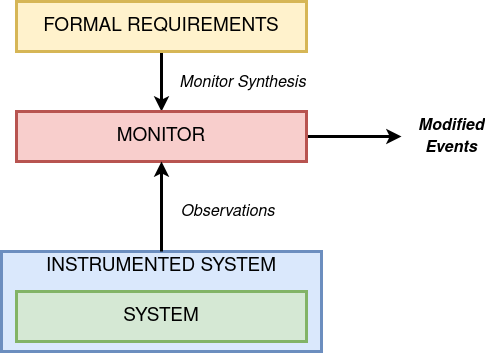
\includegraphics[width=0.6\linewidth]{av_case_study/fig/RE.png}
 \caption{An overview of the runtime enforcement process.}
    \label{fig:RE}
\end{figure}


\subsection{Enforcer Synthesis} 
\label{sec:enforcer_synthesis}

% \begin{figure}[H]
%     \centering
%     
\includegraphics[width=0.6\linewidth]{ICCPS 2024/files/fig/RE.png}
%     \caption{An overview of the runtime enforcement process}
%     \label{fig:RE}
% \end{figure}

In our work, we use the enforcer synthesis tools that are based on the approaches proposed in \cite{pearce_smart_2020,10.1145/3126500} that are suitable for safety-critical and cyber-physical systems. The framework in \cite{pearce_smart_2020} supports RE monitor synthesis for timed
policies. \gls{vdta} \cite{pearce_smart_2020} is used for the formal specification of policies, where valued signals, internal variables, and complex guard conditions are supported, ensuring compatibility with real-world CPS and industrial systems and enforcement monitors are synthesised from these \gls{vdta} to enforce a set of desired policies.\\

\noindent \textit{Prelimineries to RE.} A (finite) word is a finite sequence of elements of a finite alphabet $ \Sigma $. 
The length of $ w $ is the number of elements in $ w $ and is denoted as $ | w | $.  
%The empty word over $ \Sigma $ is denoted by $ \epsilon $. 
The sets of all words are denoted by $ \Sigma^{\ast} $. 
A language (property) over $ \Sigma $ is any subset of $ \Sigma^{\ast} $ and is denoted by $\varphi$. 

Let $\mathbb{R}$ denote the set of real numbers. $M:\mathbb{R}^n \rightarrow \mathbb{R}^m$ is a function which takes as input a vector of $n$ real valued numbers and gives as output a vector of $m$ real valued numbers. This function represents an ANN model. \\


\noindent \textit{Enforcer for $\varphi$.} An enforcer (from \cite{pearce_smart_2020}) for a property $\varphi$ is a function $E_{\varphi} : \Sigma^{\ast} \rightarrow \Sigma^{\ast}$ that takes as input a word $\Sigma^{\ast} $ and outputs a word that satisfies $\varphi$ or can be extended to satisfy $\varphi$ in the future. It can only edit an input event when necessary, and it cannot block, delay or suppress events.\\

Some constraints are required on how an enforcer transforms words. These constraints describe the expected behaviour of an enforcer and are recalled below (Def. 3.1 from \cite{10.1145/3126500}).
\begin{definition}
 Given property $\varphi$, an enforcer for $\varphi$ satisfies the following constraints:
 \begin{flushleft}
 \textbf{Soundness:}
 \end{flushleft}
        % \vspace{-1em}
 \begin{equation*}
            \label{eq:snd}
 \forall \sigma \in \Sigma^{\ast}, \exists \sigma_{extn} \in \Sigma^{\ast} : E_{\varphi} (\sigma) \cdot \sigma_{extn} \models \varphi
 \end{equation*}
        
 \begin{flushleft}
 \textbf{Monotonicity:}
 \end{flushleft}
        % \vspace{-1em}
 \begin{equation*}
            \label{eq:mo}
 \forall \sigma, \sigma_{extn} \in \Sigma^{\ast}: \sigma \preccurlyeq \sigma_{extn} \implies E_{\varphi} (\sigma) \preccurlyeq E_{\varphi} (\sigma_{extn}).
 \end{equation*} 
 where $\sigma \preccurlyeq \sigma_{extn}$ means that $\sigma$ is a prefix of $\sigma_{extn}$.

 \begin{flushleft}
 \textbf{Transparency:}
 \end{flushleft}
        % \vspace{-1em}
 \begin{equation*}
            \label{eq:tr}
 \forall \sigma, a, \sigma_{extn} \in \Sigma^{\ast} : E_{\varphi} (\sigma) \cdot a \cdot \sigma_{extn} \models \varphi \implies E_{\varphi} (\sigma \cdot a) = E_{\varphi} (\sigma) \cdot a.
 \end{equation*} 
        \label{constraints1}
\end{definition}
\vspace{-1em}
\textit{Soundness} means that for any input word, the output of the enforcer can be extended to a sequence that satisfies $\varphi$. \textit{Monotonicity} means that the output is a continuously growing word: the output of the enforcer for an extended input word $\sigma_{extn}$ of an input word $\sigma$, extends the output produced by the enforcer for $\sigma$. %i.e., for a given input word, the output can only be changed by appending new events. 
\textit{Transparency}
\footnote{\cite{pearce_smart_2020} presents a bidirectional enforcer, whereas our approach focuses on a unidirectional enforcer. Our enforcer corrects inputs from the system in a single direction and is synthesised using the monitor synthesis approach outlined in \cite{pearce_smart_2020}. Consequently, the transparency constraint defined in Def. \ref{constraints1} of our work is slightly modified compared to those in Def. 3.1 of \cite{10.1145/3126500}.} 
means that the enforcer will not unnecessarily edit any event, i.e., for any given input sequence $\sigma$ and any input event $a$, if the output of the enforcer for $\sigma$ (i.e., $E_{\varphi} (\sigma)$) followed by the input event $a$ has an extension $\sigma_{extn}$ such
that $E_{\varphi} (\sigma) \cdot a \cdot \sigma_{extn}$ satisfies the property $\varphi$, then the output that the enforcer produces for input
$\sigma \cdot a$ will be $E_{\varphi} (\sigma) \cdot a$.
    

Some other constraints are required, specifically to respect synchronous execution in reactive systems, such as \textit{instantaneity} and are recalled below (Def. 3.1 from \cite{10.1145/3126500}). 
\begin{definition}
 Given property $\varphi$, an enforcer for $\varphi$ satisfies the following constraint:
 \begin{flushleft}
 \textbf{Instantaneity:}
 \end{flushleft}
 \vspace{-1em}
 \begin{equation*}
            \label{eq:Ins}            
 \forall \sigma \in \Sigma^{\ast}: | \sigma | ~=~ | E_{\varphi} (\sigma )|
 \end{equation*}
        \label{constraints2}
\end{definition}
\vspace{-1em}
\textit{Instantaneity} means that for any given input sequence, the length of the output sequence of the enforcer should be the same as the input sequence. This means that the enforcer cannot delay, insert and suppress events. Whenever the enforcer receives a new input event, it must react instantaneously and produce an output event immediately. This requirement is essential for the enforcement of CPSs, which are reactive in nature. 


\noindent \textit{Edit Functions.} Given property $\varphi$, we introduce $edit_{\varphi}$, which the enforcer uses for
editing input events (whenever necessary) to satisfy property $\varphi$. This definition is an adapted version of the edit function presented in Section 2.2 of \cite{10.1145/3126500}. The adaptation eliminates bidirectionality, resulting in a purely unidirectional enforcer.
\begin{definition}[Edit function]
 Given an input word $\sigma \in \Sigma^{\ast}$ and an input event $x \in \Sigma$, $edit_{\varphi}(\sigma, x)$ is the set of events $x' \in \Sigma$ such that the word obtained by extending $\sigma$ with $x'$ can be extended to a sequence that satisfies the property $\varphi$ (i.e., $\exists \sigma_{extn} \in  \Sigma^{\ast}$ such that $\sigma \cdot x' \cdot \sigma_{extn} \models \varphi$). Formally,
 \begin{align*}
 edit_{\varphi}(\sigma, x) = \{x' \in \Sigma:~ \exists \sigma_{extn} \in  \Sigma^{\ast}, \sigma \cdot x' \cdot \sigma_{extn} \models \varphi\}
 \end{align*}
\end{definition}
Two proposed methods for editing non-accepting input values are given in \cite{10.1145/3126500}. These are either a random edit, where a random but accepting value would be chosen from a list of accepting values, or a minimum distance edit, where an accepting value would be chosen with minimum binary distance compared to the current
non-accepting value.

\begin{remark}[Soundness, Monotonicity, Transparency and Instantaneity]
 It has been proved that the enforcer synthesised using the approach outlined in \cite{10.1145/3126500} satisfies soundness, monotonicity, transparency and instantaneity constraints given in Def. \ref{constraints1} and \ref{constraints2}.
\end{remark}

% \saumya{sobhan, pl read}
Since our system is composed of (ML) models connected sequentially or in parallel, with an enforcer connected after the entire system, we define properties, such as \textit{inter-model consistency} and \textit{robustness}. %, which were not guaranteed without enforcers. 

%The intuition behind \textit{error containment} is that, in a compositional model, errors from one model can propagate to subsequent models, potentially compounding inaccuracies. With the \textit{sound} enforcers placed after each model \sout{in the sequence}, the system ensures that the output of each stage satisfies the local property $\varphi$. This reduces error propagation and ensures correctness at each stage.

The concept of \textit{inter-model consistency} arises from the observation that, in a decomposed ML system, multiple smaller models $M_1,\cdots M_k$ are interconnected. The output of one or more models often serves as the input to the next, forming a sequence of dependencies. The enforcer operates after the entire system, ensuring that the final output satisfies a global property $\varphi$. The intuition behind \textit{inter-model consistency} is that the relationships and dependencies between sub-models $M_1,\cdots M_k$, are conserved by the enforcer $E_{\varphi}$ even after corrections and do not contradict each other after correction.



The concept of \textit{robustness} arises from the observation that an ML model may fail to handle adversarial or unexpected inputs, potentially resulting in unsafe or unreliable behaviour. By placing an enforcer after the (decomposed) model, the system ensures operation within predefined bounds, even in scenarios that were not covered during training. In essence, an enforcer acts as a runtime safeguard in managing edge cases and adversarial inputs effectively.

\begin{definition}
 Given $n$ decomposed models $M_1, \cdots M_n$, given input vector $x_1, \cdots, x_n$ to each model and given an enforcer $E_{\varphi}$ for property $\varphi$, placed after the entire decomposed model, whose output is obtained by $E^{out}_{\varphi}$. %Let $M_i(x_i)$ denote the output of the model $M_i$ for input $x_i$ which is fed as an input to enforcer $E_i$ and let $y_{i+1}=E_i(M_i(x_i))$ denote the output of the enforcer $E_i$. 
 The system satisfies the following constraints:
    % \begin{flushleft}
    %         \textbf{Error Containment: \saumya{not correct}}
    % \end{flushleft}
    % \begin{equation*}
    %     \label{eq:ep}            
    %     \forall i \in (1,n): E_{\varphi_i}(M_i(x_i))=x_{i+1} \implies \exists \sigma_{i}' : ~x_{i+1} \cdot \sigma_{i}' \models \varphi_i
    % \end{equation*}
 \begin{flushleft}
 \textbf{Inter-model consistency:}
 \end{flushleft}
    % \begin{equation*}
    %     \label{eq:ro}            
    %     E^{out}_{\varphi} \models \varphi \implies \Bigl( \forall M_j: \{M_i, \cdots, M_k\} \rightarrow M_j \implies M_j({M_i}({x_i}^{corr})) \sim M_j(M_i(x_i)) \Bigr)
    % \end{equation*}
    % \begin{aligned}
    %      E^{out}_{\varphi} \models \varphi \implies 
    %      \Bigl( (\forall M_j: M_i \rightarrow M_j)
    %      \implies M_i \sim M_j \Bigr)\\
    %      \text{ where } M_i, M_j \in \{M_1, \cdots, M_n\}~~~~~~~~~~~~~~~~~~~~~\\
    %      \text{ where } M_1 \sim M_2 \iff (O(M_1) \land I(M_2) \neq \emptyset)~ \land \\ 
    %       ~O(M_1) \in ValidOutput(M_1) \\
    %       ~\land~I(M_2) \in ValidInput(M_2) 
    % \end{aligned}

 \begin{equation*}
 \begin{aligned}
 E^{out}_{\varphi} \models \varphi &\implies 
 \Bigl( (\forall M_j: M_i \rightarrow M_j) \implies M_i \sim M_j \Bigr) 
 \end{aligned}
 \end{equation*}
 where
 \begin{itemize}
        \item[-] $M_i, M_j \in \{M_1, \cdots, M_n\}$
        \item[-] $M_1 \sim M_2 \iff \bigl( (O(M_1) \land I(M_2) \neq \emptyset) \land~O(M_1) \in \text{ValidOutput}(M_1)  \land~I(M_2) \in \text{ValidInput}(M_2) \bigr)$
 \end{itemize} 
 \begin{flushleft}
 \textbf{Robustness:}
 \end{flushleft}
 \begin{equation*}
        \label{eq:ro}            
        % \forall \sigma_{adv_i} \in \Sigma^{\ast} \implies E_{\varphi_i}(M_i(\sigma_{adv_i})) \models \varphi_i
 \forall M_i \in \{M_1, \cdots, M_n\}, \forall \sigma_{adv} \in \Sigma^{\ast}, 
 \Bigl(M_i(\sigma_{adv})  \implies E^{out}_{\varphi} \models \varphi \Bigr)
 \end{equation*}
    \label{constraints3}
\end{definition}

%\textit{Error containment} means that there exists a potential extension $\sigma_i'$ of the output sequence $x_{i+1}$ satisfying property $\varphi_i$ at each stage. This means that for the composition of enforcers, it is ensured that each stage validates and corrects the output before it is passed to the next stage. Thus, the error propagation is reduced.

\textit{Inter-model consistency} expresses that %if $M_i$ is corrected by the enforcer to produce ${M_i}({x_i}^{corr})$, given any model $M_j$ that depends on $ M_i$'s output must still behave compatibly with how it would have behaved with the original, uncorrected output $M_i(x_i)$ provided the final enforced output $E^{out}$ satisfies property $\varphi$. 
Given a model $M_j$ whose input depends on outputs of some model $M_i$ (there can be more such models), then the relationships and dependencies between the dependent model $M_j$ and model $M_i$, are preserved by the enforcer if $\varphi$ is satisfied by the final output of the enforcer ($E^{out}_{\varphi} \models \varphi$). 

Here, $\sim$ denotes compatibility. Two models $M_1$ and $M_2$ are compatible $(M_1 \sim M_2)$ if the following conditions are met: 
(1) $M_1$'s outputs are relevant for $M_2$'s processing ($O(M_1) \land I(M_2) \neq \emptyset$);
(2) $M_1$'s outputs are valid $(O(M_1) \in ValidOutput(M_1))$;
(3) $M_2$'s inputs are valid $(I(M_2) \in ValidInput(M_2))$.
By valid, we mean that the domain and range (the structural expectations) of the input and output data remain unchanged. 
% \textcolor{red}{This ensures $M_1$ is operating correctly by producing valid outputs, which prevents the propagation of errors or invalid signals, and $M_2$ is functioning as expected by accepting inputs that are valid for its design, thus avoiding unexpected behaviour in downstream processing.}

In summary, if the enforcer guarantees that the property $\varphi$ is satisfied, then the compatibility relationship $M_i \sim M_j$ is maintained between the dependent model $M_j$ and the model $M_i$ on which it relies.\\


%\textit{Robustness} means that for any adversarial input $\sigma_{adv_i}$ the enforcer guarantees property satisfaction.
\textit{Robustness} implies that for any model $M_i$ and any adversarial input $\sigma_{adv}$, the enforcer ensures that its output satisfies the property $\varphi$ (i.e., $E^{out}_{\varphi} \models \varphi$) even when $M_i$ processes $\sigma_{adv}$.

This establishes that the enforcer effectively mitigates the impact of any adversarial inputs on the overall system behaviour, ensuring compliance with $\varphi$. 
%In simpler terms, no matter how an adversarial input impacts the models, the enforcer ensures the system adheres to the property.


\begin{proposition}[Inter-model consistency, Robustness]
 Given a property $\varphi$, its enforcer $E_{\varphi}$ satisfies Inter-model consistency and Robustness constraints as per Def. \ref{constraints3}.
    \label{propo1}
\end{proposition}
Appendix \ref{sec:proof} contains the informal proof of Proposition \ref{propo1}.







\section{Case Study}
\label{sec:case_study}
In the following subsections, we briefly explain the various modules we consider in the AV case study and define the policies we aim to enforce on these modules. Moreover, we use different models for different modules to truly represent a real-world scenario and demonstrate the flexibility of our approach.

\subsection{Case Study Modules}
\subsubsection{Lane Change Decision Module}
\label{sec:lcd_module}
The \gls{lcd} is an ML model that decides when it is opportune and safe to change lanes. We experiment with both monolithic and compositional models with various kinds of ML models. In the compositional ML model with three stages, as shown in Figure \ref{fig:3_stage_decomposition}, built as discussed in section \ref{sec:model_decomposition}, each model takes its corresponding car states and performs necessary computations to generate a decision on the lane change. 

All three models output a binary variable (0 or 1) as output, indicating whether the car should lane change or not. While the first merge block also outputs a binary decision (0 or 1), the final merge block outputs -1, 1, or 0, indicating whether the car should lane change to the left, right, or stay in the existing lane, respectively. 


\subsubsection{Car Following Module}
\label{sec:cf_module}
We use the Intelligent Driver Model (IDM) model \cite{treiber1999,PhysRevE.62.1805} for Car Following (CF). The IDM model is a car-following model that describes the dynamics of a vehicle following another vehicle. The model is based on the assumption that the vehicle follows the vehicle in front by maintaining a safe distance. The model provides the car's acceleration based on its current velocity, the distance between the vehicle and the vehicle in front, and the desired velocity. The IDM model is used in this work for its simplicity and ability to include driver preferences when modelling car-following behaviour. 

\subsubsection{Lane Change Execution Model}
\label{sec:lce_module}
The \gls{lce} model is a simple polynomial model that describes the vehicle's lateral position during a lane change. The model is based on the assumption that the vehicle changes lanes by following a polynomial trajectory. The lateral velocity is computed by taking the derivative of the polynomial that describes the lateral position as a third-degree polynomial function of time. 

\subsubsection{Controller Module}
\label{sec:controller_module}

The  \gls{av} controller operates through three primary states: Car Following (CF), Waiting (Wait), and \gls{lce}, with transitions governed by input signals, time constraints, and internal counters.

Initially, the system remains in the Car Following (CF) state unless a \gls{lcd} signal is received, indicating a left or right lane change intent. Upon receiving such a signal, the controller transitions to the Waiting (Wait) state and initialises a timer. This state is an intermediate phase to prevent abrupt transitions by ensuring the \gls{lcd} signal persists. If the signal remains active for over one second, the controller proceeds to \gls{lce}; otherwise, it reverts to Car Following (CF) if the \gls{lcd} signal returns to zero.

In the \gls{lce} state, the controller executes the lane change manoeuvre. The system remains in this state as long as the \gls{lce} signal is active. Upon completion of the lane change, when the \gls{lce} signal switches to zero, the controller transitions back to Car Following (CF), restoring its baseline operation.



\subsection{Policies}
\label{sec:policies}

\subsubsection{System-Level Policy}
\label{sec:system_level_policy}

The system-level policy for the AV case study we consider is simple. We want to ensure the AV runs safely on a freeway/motorway while executing human-like lane changes. The policy can be decomposed into two overarching sub-policies. 

\begin{itemize}
  \item $\tilde{\varphi}_{LC}$: Safe human-like lane changes
 \begin{itemize}
      \item $\tilde{\varphi}_{\gls{lcd}}$: Safe human-like lane change decision
 \begin{itemize}
        \item $\varphi_{LF}$: Safe human-like lane change decision for left front car.
        \item  $\varphi_{LP}$: Safe human-like lane change decision for left rear car.
        \item $\varphi_{RF}$: Safe human-like lane change decision for right front car.
        \item $\varphi_{RP}$: Safe human-like lane change decision for right rear car.
        \item $\varphi_{F}$: Safe human-like lane change decision for front car.
        \item $\varphi_{P}$: Safe human-like lane change decision for back car.
 \end{itemize}
      \item $\tilde{\varphi}_{\gls{lce}}$: Safe human-like lane change execution.
 \end{itemize}
  \item $\tilde{\varphi}_{CF}$: Safe Car following 
\end{itemize}


The composition of these policies ensures that the AV does not collide with any other vehicle on the road.

\begin{equation}
 \begin{aligned}
    & \tilde{\varphi}_{LC} = \tilde{\varphi}_{\gls{lcd}} \land \tilde{\varphi}_{\gls{lce}} \\
    & \tilde{\varphi} = \tilde{\varphi}_{LC} \land \tilde{\varphi}_{CF}
 \end{aligned}
\end{equation}

As the goal here is to show the compositional policy mining, training, and enforcement, we only focus on three safety policies ($\tilde{\varphi}_{\gls{lce}}, \tilde{\varphi}_{\gls{lcd}}, \tilde{\varphi}_{CF}$), one for each module, for illustration. More policies can be defined, but the composition will be similar. The following subsections define the policies in detail as a \gls{vdta}.


\subsubsection{Safety Policy for Discretionary Lane Change ($\tilde{\varphi}_{lcd}$)}
\label{sec:lcd_policy}
% \saumya{give an intuition of the policy, verbally define, then explain the parameters}


\begin{figure}[htbp]
 \begin{tikzpicture}[->,shorten >=1pt,auto,node distance=1.5cm,
 semithick,initial where=below]  
 \tikzstyle{every node}=[font=\small]
 \tikzstyle{good state}=[circle,thick,draw=blue!75,fill=blue!20,minimum size=20mm,accepting]
 \tikzstyle{bad state}=[circle,thick,draw=red!75,fill=red!20,minimum size=3mm]
 \tikzstyle{dead state}=[rectangle,thick,draw=red!75,fill=red!20,minimum size=10mm]
 \node[initial,good state] (l0) {$safe$};
 \node[dead state]         (l1) at (6,0) {$violation$};
        
 \path (l0) edge node {$\neg \varphi_{\gls{lcd}} \land \gls{lcd} $}(l1)
 (l0) edge [loop above] node { $(\varphi_{\gls{lcd}} \land \gls{lcd}) \lor (\varphi_{\gls{lcd}} \land \neg \gls{lcd})$ } (l0)    
 (l0) edge [loop left] node { $\neg \varphi_{\gls{lcd}} \land \neg \gls{lcd}$ }(l0)    
 (l1) edge  [loop above] node {$\Sigma$} (l1);
        
 \end{tikzpicture}
 \caption{Safety policy for discretionary lane change module.}
    \label{fig:lcd_policy}
\end{figure}



% \saumya{in fig, we have Plcd, in description we have P?} \sobhan{corrected}
Figure \ref{fig:lcd_policy} shows the policy for the \gls{lcd} module. Here, $ \varphi_{\gls{lcd}} = ((\varphi_{LF} \land \varphi_{LB}) \lor (\varphi_{RF} \land \varphi_{RB})) \land (\varphi_{F} \land \varphi_{CB}) $, where $\varphi_{i}$ are policies defined on car gaps and mined using Algorithm \ref{alg:compositional_training}. If $\varphi_{\gls{lcd}}=1$, it is safe to lane change, if $\varphi_{\gls{lcd}}=0$, it is not. $ \gls{lcd} = 1 $ for lane change and $\gls{lcd}=0$ for \textit{No lane change} are the possible outputs from the \gls{lcd} module. The policy says that we move to a violation state if $\varphi_{\gls{lcd}}$ is false and $\gls{lcd}$ is true, i.e. when the \gls{lcd} module's output suggests a lane change, but the policy does not think it is safe to lane change, we enter the violation state. Once we enter the violation state, we can recover by setting the $\gls{lcd}$ to 0, i.e. by making the \gls{lcd} module output a \textit{no lane change}.


\subsubsection{Safety Policy for Car Following ($\tilde{\varphi}_{CF}$)}
\label{sec:cf_policy}


\begin{figure}[htbp]
 \begin{tikzpicture}[->,shorten >=1pt,auto,node distance=3.5cm,
 el/.style = {inner sep=2pt, align=left, sloped},
 every label/.append style = {font=\small},semithick,initial where=below]
    
 \tikzstyle{every node}=[font=\small]
 \tikzstyle{good state}=[circle,thick,draw=blue!75,fill=blue!20,minimum size=20mm,accepting]
 \tikzstyle{dead state}=[rectangle,thick,draw=red!75,fill=red!20,minimum size=10mm]

    % Define states
 \node[initial,good state] (S0) {$acc$};
 \node[good state] at (8,0) (brake) {$brake$};
 \node[dead state] at (4,-5) (S3) {$violation$};

    % Transitions for s_0
 \path (S0) edge [loop left]  node {$\varphi_{CF} \land \geq 0$} (S0)
 (S0) edge node[el, above] {$\varphi_{CF} \land a < 0$} (brake)
 (S0) edge node[el, below] {$\neg \varphi_{CF} \land a \leq -u^2/2*gap$} (brake)

 (brake) edge [loop right] node {$\varphi_{CF} \land a < 0$} (brake)
 (brake) edge [loop above] node { $\neg \varphi_{CF} \land a \leq -u^2/2*gap$} (brake)
 (brake) edge [bend left] node[el, below] {$\varphi_{CF} \land a \geq 0$} (S0)

 (S0) edge node[el, below] {$\neg \varphi_{CF} \land a \geq 0$} (S3)
 (brake) edge node {$\neg \varphi_{CF} \land a > -u^2/2*gap$} (S3)
 (S3) edge [loop below] node {$\Sigma$} (S3);

 \end{tikzpicture}
 \caption{Safety policy for car following module. %Refactored safety policy with combined states.\textcolor{red}{@Partha is this okay to be kept?}
 }
    \label{fig:refactored_cf_policy_combined}
\end{figure}

Figure~\ref{fig:refactored_cf_policy_combined} presents a policy for the car following module, depicting three distinct states: \textbf{acc} (acceleration), \textbf{brake}, and \textbf{violation}. From either the \textbf{acc} or \textbf{brake} states, a transition to the \textbf{violation} state is triggered if \(\varphi_{CF}\) is false while the acceleration is non-negative in the \textbf{acc} state or if, in the \textbf{brake} state, the acceleration is greater than the critical threshold (\(a > -\frac{u^2}{2}\times gap\)). Once we enter the violation state, we can recover by setting the acceleration setpoint ($a$) to brake and equal to the $-u^2/2*gap$, which should allow the car to come to a complete stop. Here, $u$ is the velocity of the ego vehicle, $\varphi_{CF} = gap > 2m$ and $gap$ is the distance between the ego vehicle and the front vehicle.








\subsubsection{Safety Policy for Lane Change 
Execution ($\tilde{\varphi}_{lce}$)}
\label{sec:lce_policy}
\begin{figure}[htbp]
    
 \begin{tikzpicture}[->,shorten >=1pt,auto,node distance=3.5cm,el/.style = {inner sep=2pt, align=left, sloped},every label/.append style = {font=\small},semithick,initial where=left]
         
 \tikzstyle{every node}=[font=\small]
 \tikzstyle{good state}=[circle,thick,draw=blue!75,fill=blue!20,minimum size=20mm,accepting]
 \tikzstyle{bad state}=[circle,thick,draw=red!75,fill=red!20,minimum size=20mm]
 \tikzstyle{dead state}=[rectangle,thick,draw=red!75,fill=red!20,minimum size=10mm]
         
 \node[initial,good state] (S0) {$check$};
 \node[bad state] at (7,0) (S1)  {$execute$};
 % \node[dead state] (S2) [below =1 cm of S1] {$violation$};
 \node[dead state] at (7,-5)  (S2) {$violation$};
    
 \path (S0) edge node {$\gls{lce}, x:=0$}( S1)
 (S0) edge [loop above] node {$\neg \gls{lce}$} (S1)
         
 (S1) edge [bend right=60] node {$\neg \gls{lce}$} (S0)
 (S1) edge [loop above]   node {$\gls{lce}, x \leq 5$} (S1)
 (S1) edge node {$\gls{lce}, x > 5$} (S2)
 (S2) edge [loop below]   node {$\Sigma$} (S2);
 \end{tikzpicture}
\caption{Safety policy for the lane change execution module.}
\label{fig:lce_policy}
 \end{figure}
Figure \ref{fig:lce_policy} illustrates the safety policy for the \gls{lce} module. In this diagram, $\gls{lce}$ represents the Lane Change Execution signal, where $\gls{lce}=1$ indicates an ongoing lane change and $\gls{lce}=0$ indicates no active lane change. The variable $x$ tracks the duration of the lane change. The system's behaviour is described as follows: 
% \saumya{where is \gls{lcd} in fig 12? automata not correct.} \sobhan{corrected}



 

The policy states that if it takes longer than 5 seconds to complete the lane change, we enter the violation state, as something may be wrong with the execution. This time duration for a lane change is chosen based on the average lane change duration found in the real-life dataset used to train the \gls{lcd} module. If we enter the violation state, the enforcer makes the \gls{lce} signal inactive, thereby stopping the lane change execution and moving it to the Car Following state.



\section{Results}
\label{sec:results}
Once we obtain the coefficients for our mined policies and have the trained models and enforcers, we implement them in a Python simulation that mimics the ego/subject AV driving on a freeway. The results of the compositional training and the simulation are presented in this section.


\subsection{Compositional Policy-Based Training}
\label{sec:training_result}
% \saumya{policy-based training?} \sobhan{done}

We use the policy mining technique discussed in Section \ref{sec:compositional_training} to obtain the policy $\varphi_{\gls{lcd}}$ used in the \gls{lcd} enforcer. The policies are obtained using data from the well-known German highway dataset - highD \cite{krajewski_highd_2018}. We train the \gls{lcd} ML models to classify between safe ($\varphi_{\gls{lcd}}$ is satisfied ) and unsafe lane changes ($\varphi_{\gls{lcd}}$ is not satisfied). 

We experiment with three kinds of classification models in the compositional design: ANN (Artificial Neural Networks), \gls{xgb} \cite{Chen_xgboost}, and a combination of  \gls{adaboost} \cite{FREUND1997119_adaboost} and Random Forest \cite{598994_random_forest} (\gls{adaboost}+\gls{rf}) models to observe the effect of model choice. Moreover, we try four target satisfaction percentage levels (No Policy, 70\%, 80\% and 90\%) to observe their effects (from Algorithm \ref{alg:compositional_training}). \emph{No Policy} refers to a case with no policy-guided training, and a subset of the whole dataset is randomly chosen for training. 

Also, we built monolithic models with similar configurations to compare the performance of the compositional models. As our goal here is to show the effect of policies on compositional model development and enforcement, we do not tune the models to obtain optimal performance. The chosen model parameters are available in Appendix \ref{sec:appendix_model_params}.


\subsubsection{Learnt Policies}
Equation \ref{eq:lcd_policies} presents the mined policies for the model built on a 70\% satisfaction target percentage in the simulations (i.e. target percentage with the least number of faults).


\begin{equation}
\begin{aligned}
\varphi_{LF}: lfX > 80.77 + 11.23*lfV +9.72*lfA\\
\varphi_{LB}: lpX < -18.13 -2.82*lpV -2.65*lpA\\
\varphi_{RF}: rfX > 16.00 -3.21*rfV -1.51*rfA\\
\varphi_{RB}: rpX < -35.91 + 4.20*rpV -1.89*rpA\\
\varphi_{F}: fX > 0.45 + 31.14*fV -12.59*fA\\
\varphi_{B}: pX < -22.73 -1.01*pV + 4.52*pA\\
\end{aligned}
\label{eq:lcd_policies}
\end{equation}


We can observe in Equation \ref{eq:lcd_policies} that half the policies have a greater than sign and half have a less than sign. This is because the relative positions of the cars are considered in the policies, and the sign of the gap changes based on the car's position relative to the subject vehicle (i.e., car-subject car). This also explains why the front car policies have positive intercepts (the first coefficient term), and the rear/back car policies have negative intercepts. Also, we can glean from the policies that the cars, on average, need more space on the front left owing to the large positive coefficients of $\varphi_{LF}$. Other policies also show a similar behaviour.

\begin{table*}[htbp]
   \centering
   \caption{Mean 5‑fold Cross‑validation Accuracy (\%) of Models}
   \label{tab:model_performance}
   \begin{tabular}{llrrrr}
   \toprule
   \textbf{Model} & \textbf{Type} & \textbf{70} & \textbf{80} & \textbf{90} & \textbf{No Policy} \\
   \midrule
   \multirow{2}{*}{ANN} 
     & Mono & 92.073 & 91.641 & 87.060 & 71.501 \\
     & Comp & 89.500 & 89.325 & 83.168 & 66.311 \\
   \midrule
   \multirow{2}{*}{\gls{adaboost}+\gls{rf}} 
     & Mono & 91.560 & 90.645 & 87.834 & 61.061 \\
     & Comp & 90.991 & 91.201 & 87.306 & 65.821 \\
   \midrule
   \multirow{2}{*}{\gls{xgb}} 
     & Mono & 95.398 & 95.422 & 92.408 & 74.561 \\
     & Comp & 93.098 & 93.104 & 88.458 & 70.223 \\
   \bottomrule
   \end{tabular}
   \end{table*}
   


Table \ref{tab:model_performance} shows the mean accuracy of the models over the 5-fold cross-validation for all models. We can see that the accuracy of the models is generally higher for the monolithic models, except for a few cases in the \gls{adaboost}+\gls{rf} models. Statistical T-tests on the accuracies for both monolithic (Mono)  and compositional (Comp)  models also reveal that the monolithic models have a statistically higher accuracy (the p-value is 0.016 at an $\alpha$ of 5\%). It seems that the compositional models (which are architecturally more complex) do not learn the relationships in data as well as the monolithic models. Model hyperparameter tuning may help to obtain more performant compositional models. 


\subsection{Simulation Results}
\label{sec:enforcer_results}


% \begin{table*}[htbp]
%  \caption{The mean and standard deviation of the number of faults/errors that could have led to unsafe behaviour (runtime faults) over all simulation durations for the \gls{lcd} module. The mean is obtained over the 10 random simulation runs. "Mon" refers to Monolithic, and "Comp" refers to Compositional models.}
%  \begin{tabular}{c|cccc|cccc|cccc}
%  \toprule
%  {} & \multicolumn{4}{c}{ANN} & \multicolumn{4}{c}{\gls{adaboost}+\gls{rf}} & \multicolumn{4}{c}{\gls{xgb}} \\
%  {} & \multicolumn{2}{c}{Mono} & \multicolumn{2}{c}{Comp} & \multicolumn{2}{c}{Mono} & \multicolumn{2}{c}{Comp} & \multicolumn{2}{c}{Mono} & \multicolumn{2}{c}{Comp} \\
%  {} & mean & std & mean & std & mean & std & mean & std & mean & std & mean & std \\
%  \midrule
%  70   & 43.150 & 16.158 & 7.200 & 0.000 & 3.600 & 0.000 & 9.500 & 0.000 & 10.100 & 0.000 & 9.200 & 0.000 \\
%  80   & 107.275 & 62.251 & 2.800 & 0.000 & 3.200 & 0.000 & 3.200 & 0.000 & 4.900 & 0.000 & 3.400 & 0.000 \\
%  90   & 307.800 & 195.716 & 8.950 & 0.141 & 738.487 & 472.865 & 626.112 & 374.425 & 293.988 & 183.176 & 392.100 & 221.362 \\
%  No Policy & 43.150 & 16.158 & 19.875 & 8.896 & 743.550 & 470.663 & 585.400 & 366.411 & 957.200 & 610.441 & 466.350 & 299.387 \\
%  \bottomrule
%  \end{tabular}
%         \label{tab:sim_lcd}
% \end{table*}

\begin{table*}[htbp]
   \centering
   \caption{Mean and standard deviation of runtime faults for the \gls{lcd} module (10 runs).}
   \label{tab:sim_lcd}
   \begin{tabular}{lllrrrr}
   \toprule
   \textbf{Model} & \textbf{Type}     & \textbf{Statistic} & \textbf{70}   & \textbf{80}   & \textbf{90}    & \textbf{No Policy} \\ 
   \midrule
   \multirow{4}{*}{ANN} 
     & \multirow{2}{*}{Mono} & mean &  43.150 & 107.275 & 307.800 &  43.150 \\
     &                       & std  &  16.158 &  62.251 & 195.716 &  16.158 \\ 
     & \multirow{2}{*}{Comp} & mean &   7.200 &   2.800 &   8.950 &  19.875 \\
     &                       & std  &   0.000 &   0.000 &   0.141 &   8.896 \\ 
   \midrule
   \multirow{4}{*}{\gls{adaboost}+\gls{rf}} 
     & \multirow{2}{*}{Mono} & mean &   3.600 &   3.200 & 738.487 & 743.550 \\
     &                       & std  &   0.000 &   0.000 & 472.865 & 470.663 \\ 
     & \multirow{2}{*}{Comp} & mean &   9.500 &   3.200 & 626.112 & 585.400 \\
     &                       & std  &   0.000 &   0.000 & 374.425 & 366.411 \\ 
   \midrule
   \multirow{4}{*}{\gls{xgb}} 
     & \multirow{2}{*}{Mono} & mean &  10.100 &   4.900 & 293.988 & 957.200 \\
     &                       & std  &   0.000 &   0.000 & 183.176 & 610.441 \\ 
     & \multirow{2}{*}{Comp} & mean &   9.200 &   3.400 & 392.100 & 466.350 \\
     &                       & std  &   0.000 &   0.000 & 221.362 & 299.387 \\ 
   \bottomrule
   \end{tabular}
   \end{table*}
   

The simulation setup used to evaluate the trained models and enforcers is described in Section \ref{sec:simulation_setup}. We inject faults at regular intervals in the simulation to observe the behaviour of the AV under simulated unsafe conditions. The modules may also produce unsafe behaviour on their own, which we call runtime faults. During both unsafe behaviours (recorded over 10 random iterations), we expect the enforcer to act and take corrective action. We report these observations as follows.

We can see from Table \ref{tab:sim_lcd} that the \gls{lcd} module, which is composed of ML models, produced several runtime faults (total faults-injected faults) that activated the \gls{lcd} enforcer. The number of faults varied across the different configurations of the compositional training. However, the number of faults is generally lower for the compositional models. This observation suggests a trade-off between the number of enforcer activations and the policy satisfaction target percentage. In particular, it can be seen that too high a target percentage and too low a target percentage (No Policy dataset) can lead to more enforcer activations, indicating that the model overfits the training data and cannot generalise well if the target percentage is too high or too low. 

We also perform a statistical T-test on the \gls{lcd} model faults to determine if there is a statistical difference between the values of the monolithic and compositional models. The T-test results show that the compositional models have a statistically significantly lower number of faults  (with a p-value of 0.034 at an $\alpha$ of 5\%) than the monolithic models. We also test the difference between faults seen in the policy and the No Policy models. The T-test results show that the N Policy models have a statistically significantly higher number of faults  (with a p-value of 0.034 at an $\alpha$ of 5\%). We also find that the statistical effect sizes measured using Cohen's d are moderate to high, suggesting that the differences in faults are meaningful. This result suggests that the compositional models (resp. policy trained models) are better at generalising to unseen data than the monolithic (resp. No Policy trained) models and ensuring safer behaviour.


Additionally, the CF module, which is a stateful mathematical model, produced far fewer runtime faults compared to the ML-based \gls{lcd} module. The mean number of faults over the ten random simulation runs is 0.187. The simple deterministic nature of the CF module, which is governed by strict mathematical rules, does not have the same generalisation issues as the ML models. Similarly, the mathematical \gls{lce} polynomial model produced no runtime faults in the simulation run. The number of injected faults is the same for all modules.

We also observe from the simulation logs (which we do not present here for brevity) that the gaps between cars do not become zero at any point for all cases considered, indicating that the enforcers' corrective actions are sufficient to maintain safe behaviour. The logs also show that the subject vehicle executes lane changes where appropriate and does not get stuck in deadlock situations where the vehicle does not know what to do. We do not report these results numerically for brevity.



\subsection{Discussion}
\label{sec:av_results_discussion}

The training and simulation results show a clear split between predictive metrics on held-out cross-validation and safety-related behaviour under fault injection. Table~\ref{tab:model_performance} indicates that monolithic models achieve higher classification accuracy than compositional models for ANN and \gls{xgb} ($p = 0.016$). Table~\ref{tab:sim_lcd}, however, shows fewer runtime faults for compositional models in most configurations ($p = 0.034$), and policy-guided training yields fewer faults than the No Policy baseline. ML-based modules are therefore prone to unsafe runtime behaviour when policies are not used to shape training, even when accuracy appears strong. By contrast, the mathematical car-following and lane-change execution modules produce far fewer faults (mean 0.187 and zero runtime faults, respectively), reflecting their deterministic structure, but they depend on assumptions about module behaviour and offer less flexibility to learn variability from data.

For the \gls{lcd} module specifically, the lower fault counts of compositional, policy-trained models suggest that classification accuracy alone is not a reliable indicator of how the system will behave when disturbances are injected. Compositional architectures together with policy-filtered datasets emphasise adherence to mined gap conditions; this appears to generalise better under simulation stress than maximising accuracy on the cross-validation split. The trade-off between target satisfaction percentage and faults is also visible in the results: very high or very low targets (90\% or No Policy) tend to coincide with more enforcer activations, whereas the 70\% setting used for the policies in Equation~\ref{eq:lcd_policies} balances fit to highD and stable runtime behaviour.

The mined coefficients in Equation~\ref{eq:lcd_policies} illustrate how empirical data refines, rather than replaces, the policy structure fixed in Section~\ref{sec:compositional_training}. Each predicate keeps a kinematic template; highD trajectories determine the numerical thresholds. Because leaf models are trained for approximate satisfaction of sub-formulae and coefficients are themselves empirical estimates, system-level safety cannot be obtained by composing per-leaf satisfaction rates in closed form. The simulation outcomes provide the practical assessment instead: policy-trained compositional models reduce faults, simulation logs maintain non-zero gaps between vehicles, and the \gls{lcd} enforcer corrects residual violations at runtime. Together with the workflow in Section~\ref{sec:model_decomposition}---mine constituents, compose models, evaluate with enforcement---these results show how approximate local policies can still support dependable end-to-end behaviour when validation moves from static accuracy to dynamic simulation.

The structure of the \gls{lcd} decomposition also explains why the framework is applicable in some pipeline settings but not all. Within the decision module, $\varphi_{\gls{lcd}}$ is split into left, right, and opportunity sub-formulae (Figure~\ref{fig:3_stage_decomposition}) because each predicate refers to a distinct aspect of the same traffic configuration $y$. Where safety depends on the output of an upstream module, the case study assigns separate policies to \gls{lcd}, \gls{lce}, and car following and applies enforcement on the final control output in the serial simulation described in Section~\ref{sec:simulation_setup}. The comparatively low fault rate of the non-ML modules indicates that compositional policy training and runtime enforcement add the most value alongside learning-based components, which dominate the residual risk observed in Table~\ref{tab:sim_lcd}.

The three-leaf \gls{lcd} layout follows driving semantics (lateral direction and opportunity) rather than an exhaustive search over alternative partitions; a six-leaf design per atomic gap condition was not evaluated here. The simulation supports the chosen decomposition but does not rule out other architectures. Overall, the results indicate that a lightweight runtime enforcement layer, combined with compositional policy-based training, can improve safety relative to monolithic and unguided training while accepting a modest reduction in cross-validation accuracy. Policy mining remains limited to linear templates in this chapter, and broader validation on additional datasets would strengthen claims about generalisability.


\section{Summary}
\label{sec:av_summary}

In this chapter, we introduced a model-agnostic policy-driven approach to compositional ML-based safety-critical \glspl{cps}. Given policy templates and data, we mine compositional properties, train compositional ML models (\gls{ann}, \gls{xgb}, \gls{adaboost}+\gls{rf}) under satisfaction tolerances, and deploy runtime enforcers. We validated the framework on an AV simulation with lane-change decision, lane-change execution, and car-following modules.

The methodology extracts meaningful linear policies from highD, and simulation shows that policy-based compositional training reduces unsafe runtime behaviour compared with monolithic and No Policy training, with enforcers maintaining safe gaps. Limitations include linear policy templates, manual decomposition choices, and the scope of the single case study. Future work includes richer policy classes, tighter integration of mining and training, and broader evaluation on additional datasets and domains.




